\documentclass[12pt]{article}

\usepackage{sbc-template}

\usepackage[brazil]{babel}
\usepackage[utf8]{inputenc}
\usepackage{graphicx}
\usepackage{amsmath}
\usepackage{url}
\usepackage{booktabs}

\sloppy

\title{Predição de $\lambda_{max}$ de Moléculas Orgânicas via Aprendizado Profundo: Comparação de Arquiteturas e Aplicação em Triagem Computacional}

\author{Crhisângela Ferreira\inst{1}}

\address{Programa de Pós-Graduação em Ciência da Computação\\
  Universidade Federal do ABC (UFABC)\\
  CCM-109 -- Tópicos Especiais em Inteligência Artificial
  \email{crhisangela.ferreira@ufabc.edu.br}
}

\begin{document}

\maketitle

\begin{resumo}
A predição do comprimento de onda de máxima absorção ($\lambda_{max}$) de moléculas orgânicas é relevante para o desenvolvimento de corantes, sensores e fotocatalisadores, mas métodos quânticos de referência (DFT) têm custo computacional elevado para triagens em larga escala. Este trabalho treina e compara três abordagens obrigatórias (-- )MLP com fingerprints Morgan, Gradient Boosting sobre descritores RDKit e Bi-LSTM bidirecional sobre SMILES), além de uma extensão opcional de estado da arte (D-MPNN/Chemprop), para prever $\lambda_{max}$ a partir do SMILES do cromóforo e do solvente, usando o dataset público Deep4Chem. O melhor modelo é então aplicado, com quantificação de incerteza (MC-Dropout ou ensemble bootstrap, conforme o modelo), a um conjunto proprietário de 5.974 moléculas geradas computacionalmente, para priorizar candidatos à síntese experimental. Em uma execução preliminar de validação do pipeline (subamostra reduzida do Deep4Chem), o Gradient Boosting obteve o melhor desempenho (MAE de 44,5 nm no teste), e a análise de deslocamento de distribuição revelou diferenças estatisticamente significativas entre o Deep4Chem e o conjunto proprietário, sinalizando cautela na transferência do modelo.
\end{resumo}

\begin{abstract}
Predicting the wavelength of maximum absorption ($\lambda_{max}$) of organic molecules is relevant for the development of dyes, sensors and photocatalysts, but reference quantum-chemical methods (DFT) are computationally expensive for large-scale screening. This work trains and compares three required approaches -- an MLP over Morgan fingerprints, Gradient Boosting over RDKit descriptors, and a bidirectional LSTM over SMILES --, plus an optional state-of-the-art extension (D-MPNN/Chemprop), to predict $\lambda_{max}$ from the chromophore and solvent SMILES, using the public Deep4Chem dataset. The best model is then applied, with uncertainty quantification (MC-Dropout or bootstrap ensembling, depending on the model), to a proprietary set of 5,974 computationally generated molecules, in order to prioritize candidates for experimental synthesis. In a preliminary pipeline-validation run (reduced subsample of Deep4Chem), Gradient Boosting achieved the best performance (test MAE of 44.5 nm), and the distribution-shift analysis revealed statistically significant differences between Deep4Chem and the proprietary set, indicating that model transfer should be treated with caution.
\end{abstract}

\section{Descrição do Problema}

A predição de propriedades ópticas de moléculas orgânicas é um desafio central em quimioinformática e no desenvolvimento de novos materiais. Em particular, o comprimento de onda de máxima absorção ($\lambda_{max}$) no espectro UV-Vis determina aplicações em corantes, sensores e fotocatalisadores. Métodos quânticos baseados na Teoria do Funcional da Densidade (DFT) \cite{hohenberg1964,kohnsham1965}, em sua formulação dependente do tempo (TD-DFT) \cite{adamo2013}, permitem calcular estados excitados e $\lambda_{max}$ com boa precisão, mas seu custo computacional elevado inviabiliza a triagem em larga escala sobre espaços moleculares amplos.

Este trabalho formula o problema como uma tarefa de regressão supervisionada: dado o SMILES de um cromóforo e o SMILES do solvente em que ele é medido, prever o valor de $\lambda_{max}$ (em nanômetros). A escolha de incluir o solvente como entrada decorre do fato de que $\lambda_{max}$ é sensível ao ambiente químico (efeitos solvatocrômicos) \cite{reichardt1994}, e não apenas à estrutura do cromóforo isolado.

O projeto é dividido em duas etapas. Na Etapa 1, modelos são treinados e comparados sobre um dataset público rotulado, com o objetivo de identificar a abordagem com melhor generalização. Na Etapa 2, o modelo selecionado é aplicado como ferramenta de triagem exploratória sobre um conjunto proprietário de 5.974 moléculas sem rótulo, geradas computacionalmente por um aluno de iniciação científica do laboratório ABC Sim da UFABC, produzindo um ranking de candidatos prioritários para síntese experimental.

\subsection{Motivação}

A motivação prática do projeto é substituir, para fins de triagem inicial, cálculos DFT custosos por um modelo de aprendizado de máquina treinado sobre dados experimentais, capaz de gerar predições em escala para milhares de moléculas em segundos. Isso é particularmente relevante para o laboratório ABC Sim, que já dispõe de um espaço de moléculas geradas computacionalmente e precisa de um critério eficiente para priorizar quais estruturas sintetizar e caracterizar experimentalmente.

\subsection{Definição Formal da Tarefa}

Seja $s_c$ o SMILES do cromóforo e $s_v$ o SMILES do solvente. O objetivo é aprender uma função $f(s_c, s_v) \rightarrow \hat{y}$, em que $\hat{y}$ é a predição de $\lambda_{max}$ em nanômetros, minimizando o Erro Médio Absoluto (MAE) entre $\hat{y}$ e o valor experimental $y$ em um conjunto de teste mantido separado do treino.

\section{Abordagem}

\subsection{Conjunto de Dados}

O treinamento e a avaliação dos modelos são realizados sobre o Deep4Chem \cite{joung2020}, base de dados pública disponível via Figshare (DOI: 10.6084/m9.figshare.12045567.v2). O Deep4Chem compila propriedades ópticas experimentais de 7.016 cromóforos orgânicos únicos medidos em 365 solventes distintos, totalizando 20.236 registros extraídos de 1.358 artigos científicos. Cada entrada contém o SMILES do cromóforo, o SMILES do solvente, $\lambda_{abs}$, $\lambda_{em}$, coeficiente de extinção molar e rendimento quântico; para este trabalho, apenas o SMILES do cromóforo, o SMILES do solvente e $\lambda_{abs}$ (renomeado \texttt{lambda\_max}) são utilizados.

Na Etapa 2, o modelo treinado é aplicado sobre o conjunto proprietário de 5.974 moléculas (\texttt{resources/banco\_smiles\_aromatizados.parquet}), representadas por SMILES canônicos e por colunas de identificação que rastreiam os anéis/fragmentos de origem de cada molécula. Esse conjunto não possui rótulos de $\lambda_{max}$ e é usado exclusivamente para triagem exploratória, nunca para treino ou avaliação.

\subsection{Pré-processamento}

Os SMILES do Deep4Chem são validados com o RDKit \cite{rdkit2024} (\texttt{Chem.MolFromSmiles}), descartando-se registros com valores ausentes ou SMILES inválidos, e removendo-se duplicatas por par (cromóforo, solvente). Como $\lambda_{max}$ depende do solvente, o SMILES do solvente é mantido como feature em todos os modelos, e não descartado no pré-processamento.

\textbf{Parsing tolerante do conjunto proprietário.} Ao contrário do Deep4Chem, aproximadamente metade dos SMILES do conjunto proprietário usa notação de aromaticidade explícita com o símbolo \texttt{:} entre átomos maiúsculos (não aromáticos na notação padrão), o que faz o parser padrão do RDKit falhar ao tentar kekulizar a molécula (\textit{Can't kekulize mol}). Para esses casos, o notebook refaz o parsing com \texttt{sanitize=False} seguido de \texttt{Chem.SanitizeMol} com a flag \texttt{SANITIZE\_KEKULIZE} desabilitada, preservando a informação de aromaticidade sem exigir uma estrutura de Kekulé explícita. Essa estratégia elevou a taxa de parsing do conjunto proprietário de $\approx$49\% para 100\% (5.974/5.974 moléculas).

\textbf{Divisão dos dados (scaffold split).} Em vez de uma divisão aleatória entre treino e teste, é adotado um \textit{scaffold split} por molécula, baseado no arcabouço de Bemis-Murcko \cite{bemis1996}: todas as ocorrências de uma mesma família estrutural (scaffold) do cromóforo são mantidas inteiramente no treino ou inteiramente no teste (80\%/20\%). Essa escolha evita que o mesmo esqueleto molecular apareça em treino e teste, o que superestimaria a capacidade de generalização do modelo caso fosse usada uma divisão aleatória -- recomendação incorporada a partir do feedback recebido sobre a proposta inicial do projeto.

\subsection{Modelos}

São implementadas e comparadas três abordagens obrigatórias, todas em PyTorch \cite{paszke2019}/scikit-learn \cite{pedregosa2011}:

\begin{itemize}
  \item \textbf{Baseline 1 -- MLP com fingerprints Morgan.} Os SMILES do cromóforo e do solvente são convertidos em vetores binários via fingerprints de Morgan \cite{rogers2010} (2.048 bits para o cromóforo, 256 bits para o solvente, raio 2, calculados com RDKit) e concatenados como entrada de uma rede totalmente conectada (MLP) com camadas ocultas de até 512 e 256 unidades, ativação ReLU e \textit{dropout} \cite{srivastava2014}.
  \item \textbf{Baseline 2 (forte) -- Gradient Boosting sobre descritores RDKit.} Um \texttt{GradientBoostingRegressor} \cite{friedman2001} é treinado sobre $\approx$217 descritores físico-químicos calculados pelo RDKit (peso molecular, LogP, número de anéis aromáticos, TPSA, cargas parciais, entre outros) \cite{todeschini2009}, computados tanto para o cromóforo quanto para o solvente -- incorporado como comparação adicional sugerida no feedback da proposta.
  \item \textbf{Modelo principal -- Bi-LSTM \textit{char-level}.} Cada caractere do SMILES do cromóforo é mapeado a um \textit{embedding} treinável e processado por uma LSTM bidirecional \cite{hochreiter1997,schuster1997}; a concatenação dos últimos estados forward/backward é combinada ao fingerprint Morgan do solvente (256 bits) antes de passar por camadas densas que produzem a predição final.
  \item \textbf{Extensão opcional -- D-MPNN (Chemprop).} Uma rede de mensagens direcionadas sobre o grafo molecular \cite{gilmer2017,yang2019}, na linha dos benchmarks de aprendizado molecular consolidados pelo MoleculeNet \cite{wu2018}, incluída como comparação de estado da arte em uma célula separada e autocontida do notebook (\texttt{RUN\_CHEMPROP=True}), condicionada à disponibilidade da biblioteca \texttt{chemprop} e de tempo de treino antes da entrega.
\end{itemize}

\subsection{Protocolo Experimental}

Todos os modelos obrigatórios são avaliados com o mesmo scaffold split (80\% treino / 20\% teste), e a métrica principal reportada é o Erro Médio Absoluto (MAE, em nm), complementada pela Raiz do Erro Quadrático Médio (RMSE, em nm) -- ambas incorporadas a partir da recomendação de reportar as duas métricas em vez de apenas o MAE. Hiperparâmetros (tamanho da camada oculta e \textit{dropout} do MLP; profundidade e taxa de aprendizado do GBM; dimensão do \textit{embedding} e da camada oculta da Bi-LSTM) são selecionados por validação cruzada em grupos de scaffold (\texttt{GroupKFold} agrupado pelo mesmo scaffold de Bemis-Murcko do split externo), evitando que a mesma família estrutural apareça simultaneamente em treino e validação de um fold.

\subsection{Etapa 2 -- Aplicação e Quantificação de Incerteza}

O modelo com melhor desempenho na Etapa 1 é aplicado ao conjunto proprietário de 5.974 moléculas para gerar um ranking de $\lambda_{max}$ previsto. Como esse conjunto não possui um solvente rotulado, é adotado como referência constante o solvente mais frequente no Deep4Chem (diclorometano, \texttt{ClCCl}) -- decisão que deve ser ajustada conforme o contexto experimental real do laboratório ABC Sim.

Como esse ranking guiará decisões de síntese experimental, foi incorporada quantificação de incerteza, escolhida de acordo com o tipo do modelo vencedor: para os modelos neurais (MLP ou Bi-LSTM), usa-se \textbf{MC-Dropout} \cite{gal2016,srivastava2014} -- o modelo é mantido em modo de treinamento (\textit{dropout} ativo) durante a inferência, e múltiplas passadas sobre a mesma molécula produzem uma distribuição de predições cujo desvio-padrão é usado como proxy de incerteza; para o Gradient Boosting, que não possui \textit{dropout}, é treinado em seu lugar um pequeno \textbf{ensemble bootstrap} de modelos com os mesmos hiperparâmetros, sementes e subamostras (\texttt{subsample}) distintas, na linha de ensembles preditivos para quantificação de incerteza \cite{lakshminarayanan2017}, cuja dispersão de predições cumpre o mesmo papel. Em ambos os casos, candidatos de alta confiança (baixa variância entre passadas/modelos) são priorizados no ranking final. Também é realizada uma análise de deslocamento de distribuição (\textit{domain shift}) entre o Deep4Chem e o conjunto proprietário, comparando estatísticas de descritores moleculares-chave (peso molecular, LogP, TPSA, doadores/aceptores de ligação de hidrogênio, anéis aromáticos, ligações rotacionáveis) por meio do teste de Kolmogorov-Smirnov, para avaliar até que ponto a transferência do modelo é confiável.

\section{Resultados}

\textbf{Nota sobre o status dos resultados.} Os números desta seção foram obtidos em uma execução de \textbf{validação do pipeline} (\texttt{QUICK\_TEST=True} no notebook), sobre uma subamostra de 1.500 registros do Deep4Chem e com um número reduzido de épocas de treino, com o único objetivo de confirmar que o código roda de ponta a ponta sem erros antes da execução completa. Eles \textbf{não} são os resultados finais do projeto -- a execução completa (\texttt{QUICK\_TEST=False}, dataset inteiro, Google Colab com GPU) ainda precisa ser realizada e deve substituir as tabelas abaixo antes da entrega final. Ainda assim, os resultados preliminares já são informativos e são discutidos como tal.

\subsection{Comparação entre modelos (Etapa 1)}

A Tabela \ref{tab:comparacao} mostra o desempenho dos três modelos obrigatórios no conjunto de teste (scaffold split), na execução preliminar sobre 1.500 registros (1.216 de treino / 284 de teste, 0 scaffolds em comum entre os conjuntos).

\begin{table}[h]
\centering
\caption{Comparação de desempenho dos modelos na Etapa 1 (conjunto de teste, scaffold split) -- resultado preliminar, subamostra de validação do pipeline.}
\label{tab:comparacao}
\begin{tabular}{lcc}
\toprule
Modelo & MAE (nm) & RMSE (nm) \\
\midrule
Gradient Boosting (descritores RDKit) & \textbf{44,5} & \textbf{60,5} \\
MLP + fingerprints Morgan & 51,1 & 70,7 \\
Bi-LSTM (SMILES + solvente) & 81,5 & 109,8 \\
D-MPNN (Chemprop, opcional) & -- & -- \\
\bottomrule
\end{tabular}
\end{table}

\begin{figure}[h]
\centering
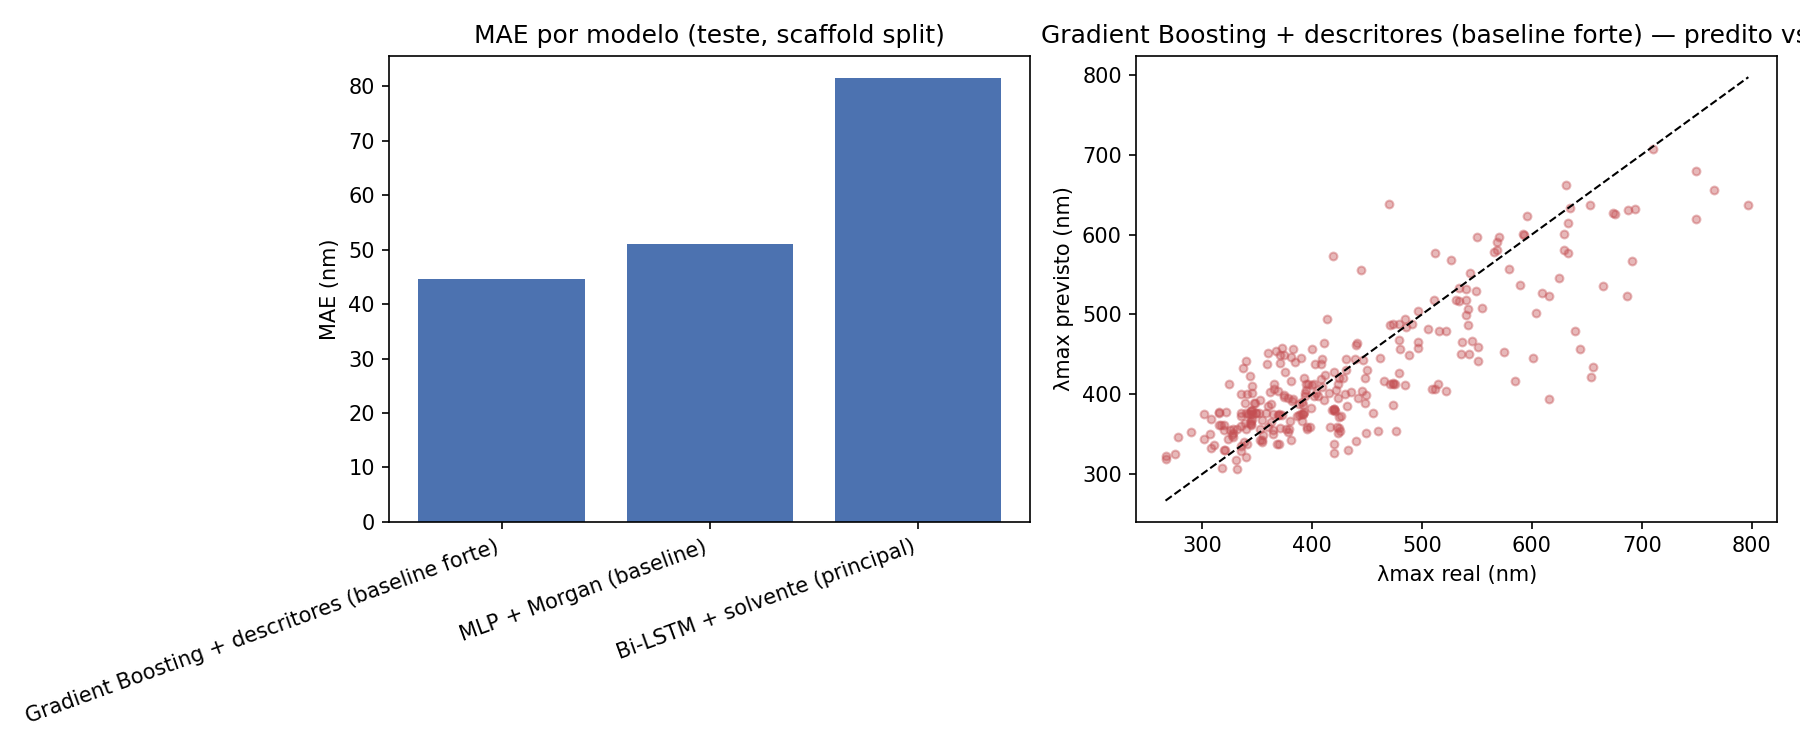
\includegraphics[width=\textwidth]{../resources/figures/comparacao_modelos.png}
\caption{Esquerda: MAE de teste por modelo. Direita: dispersão $\lambda_{max}$ previsto vs. real para o melhor modelo (Gradient Boosting) -- resultado preliminar (subamostra de validação).}
\label{fig:comparacao}
\end{figure}

Nessa rodada reduzida, o \textbf{Gradient Boosting} superou tanto o MLP quanto a Bi-LSTM. Os descritores RDKit mais importantes para o modelo foram, em ordem: \texttt{MaxAbsPartialCharge}, \texttt{NumAliphaticHeterocycles}, \texttt{fr\_allylic\_oxid}, \texttt{SMR\_VSA10}, \texttt{BCUT2D\_MRLOW}, \texttt{PEOE\_VSA8}, \texttt{BertzCT}, \texttt{MinPartialCharge}, \texttt{Chi3n} e \texttt{NumAliphaticRings} -- coerente com a expectativa química de que cargas parciais e complexidade estrutural/eletrônica estão associadas à posição de $\lambda_{max}$. A Bi-LSTM, apesar de ser o modelo principal proposto, teve o pior desempenho nessa execução reduzida; a hipótese mais provável (a ser confirmada na execução completa, ver Seção 4) é que redes neurais treinadas do zero sobre representações \textit{char-level} exigem mais dados e épocas para convergir do que uma subamostra de 1.216 moléculas de treino permite.

\subsection{Etapa 2 -- Ranking e incerteza}

O modelo vencedor da Etapa 1 nessa rodada preliminar (Gradient Boosting) foi aplicado às 5.974 moléculas do conjunto proprietário, com o solvente de referência constante \texttt{ClCCl} (diclorometano) e quantificação de incerteza por ensemble bootstrap (5 modelos). A Tabela \ref{tab:etapa2} resume a distribuição do $\lambda_{max}$ previsto e da incerteza (desvio-padrão entre modelos do ensemble); a Figura \ref{fig:etapa2} mostra a distribuição do ranking e a relação entre $\lambda_{max}$ previsto e incerteza.

\begin{table}[h]
\centering
\caption{Estatísticas descritivas do ranking de $\lambda_{max}$ previsto para as 5.974 moléculas proprietárias -- resultado preliminar.}
\label{tab:etapa2}
\begin{tabular}{lcc}
\toprule
Estatística & $\lambda_{max}$ previsto (nm) & Incerteza -- desvio padrão (nm) \\
\midrule
Média & 466,4 & 21,5 \\
Desvio padrão & 53,2 & 7,4 \\
Mínimo & 321,8 & 2,3 \\
1º quartil & 428,6 & 16,3 \\
Mediana & 464,2 & 21,2 \\
3º quartil & 503,2 & 26,4 \\
Máximo & 670,0 & 51,2 \\
\bottomrule
\end{tabular}
\end{table}

\begin{figure}[h]
\centering
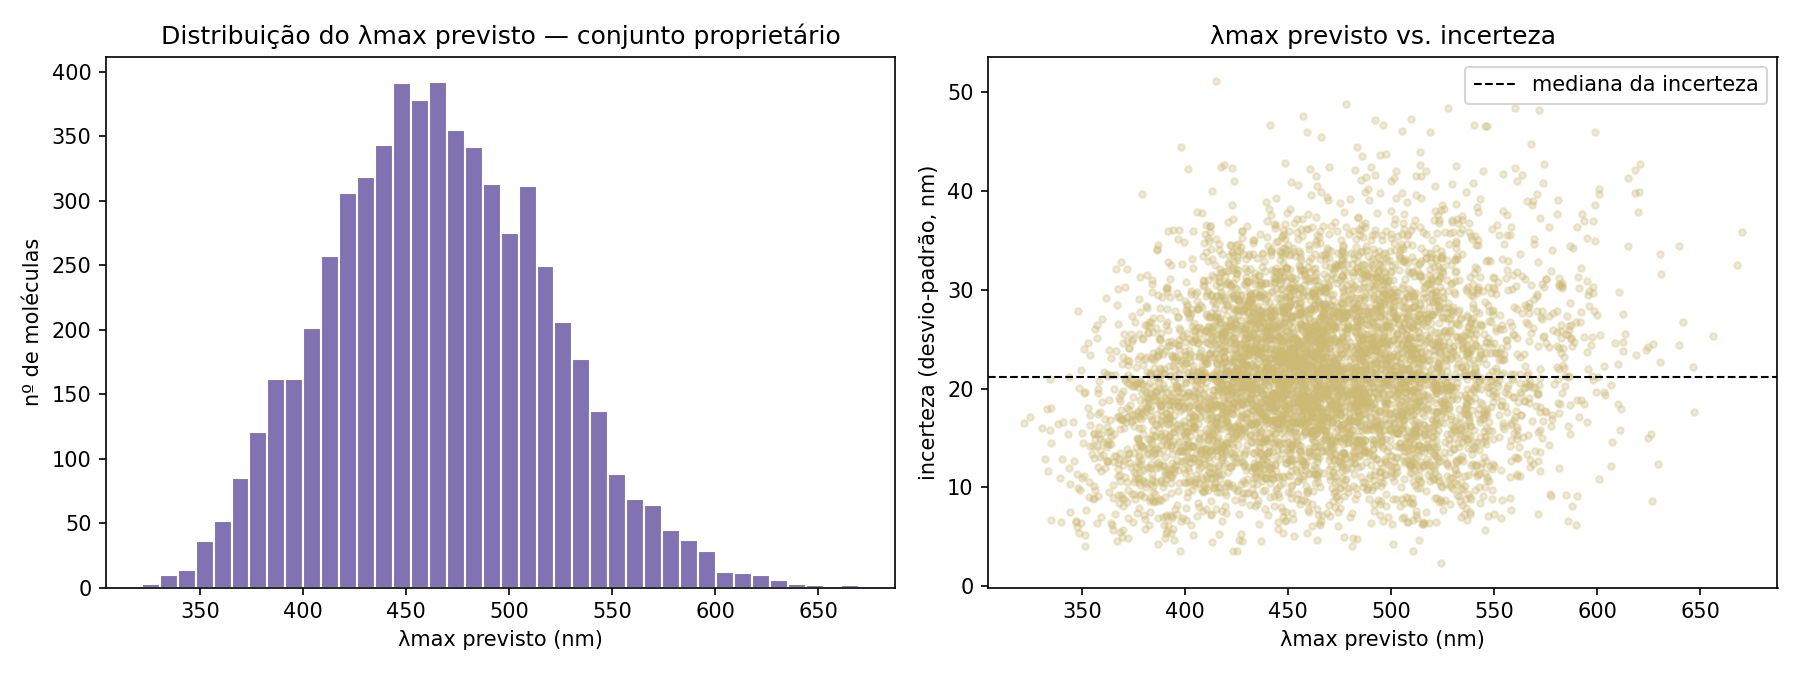
\includegraphics[width=\textwidth]{../resources/figures/etapa2_ranking_incerteza.png}
\caption{Esquerda: distribuição do $\lambda_{max}$ previsto para o conjunto proprietário. Direita: $\lambda_{max}$ previsto vs. incerteza, com a mediana da incerteza como referência para a triagem de candidatos de alta confiança -- resultado preliminar.}
\label{fig:etapa2}
\end{figure}

Os candidatos prioritários para síntese são selecionados combinando alto $\lambda_{max}$ previsto \textbf{e} incerteza abaixo da mediana; entre os 15 candidatos de maior $\lambda_{max}$ previsto nessas condições, os valores variam entre 600 e 647 nm, com incerteza entre 8,6 e 21,2 nm. O ranking completo, com as colunas de proveniência (anéis/fragmentos de origem), é exportado em \texttt{resources/ranking\_lambda\_max\_proprietario.csv} para uso direto pelo laboratório ABC Sim.

\subsection{Deslocamento de distribuição (\textit{domain shift})}

A Tabela \ref{tab:domainshift} e a Figura \ref{fig:domainshift} comparam a distribuição de sete descritores moleculares-chave entre os cromóforos de treino do Deep4Chem e as moléculas do conjunto proprietário, via teste de Kolmogorov-Smirnov (hipótese nula: mesma distribuição).

\begin{table}[h]
\centering
\caption{Deslocamento de distribuição entre o Deep4Chem (treino) e o conjunto proprietário -- resultado preliminar, ordenado por estatística KS decrescente. Todos os $p$-valores $< 10^{-180}$.}
\label{tab:domainshift}
\begin{tabular}{lccc}
\toprule
Descritor & Média Deep4Chem & Média proprietário & KS \\
\midrule
NumHAcceptors & 3,45 & 8,81 & 0,747 \\
TPSA & 50,35 & 148,06 & 0,745 \\
NumHDonors & 0,49 & 3,13 & 0,737 \\
NumAromaticRings & 4,21 & 0,92 & 0,714 \\
MolLogP & 6,51 & 1,39 & 0,618 \\
NumRotatableBonds & 5,10 & 8,53 & 0,531 \\
MolWt & 456,15 & 524,57 & 0,448 \\
\bottomrule
\end{tabular}
\end{table}

\begin{figure}[h]
\centering
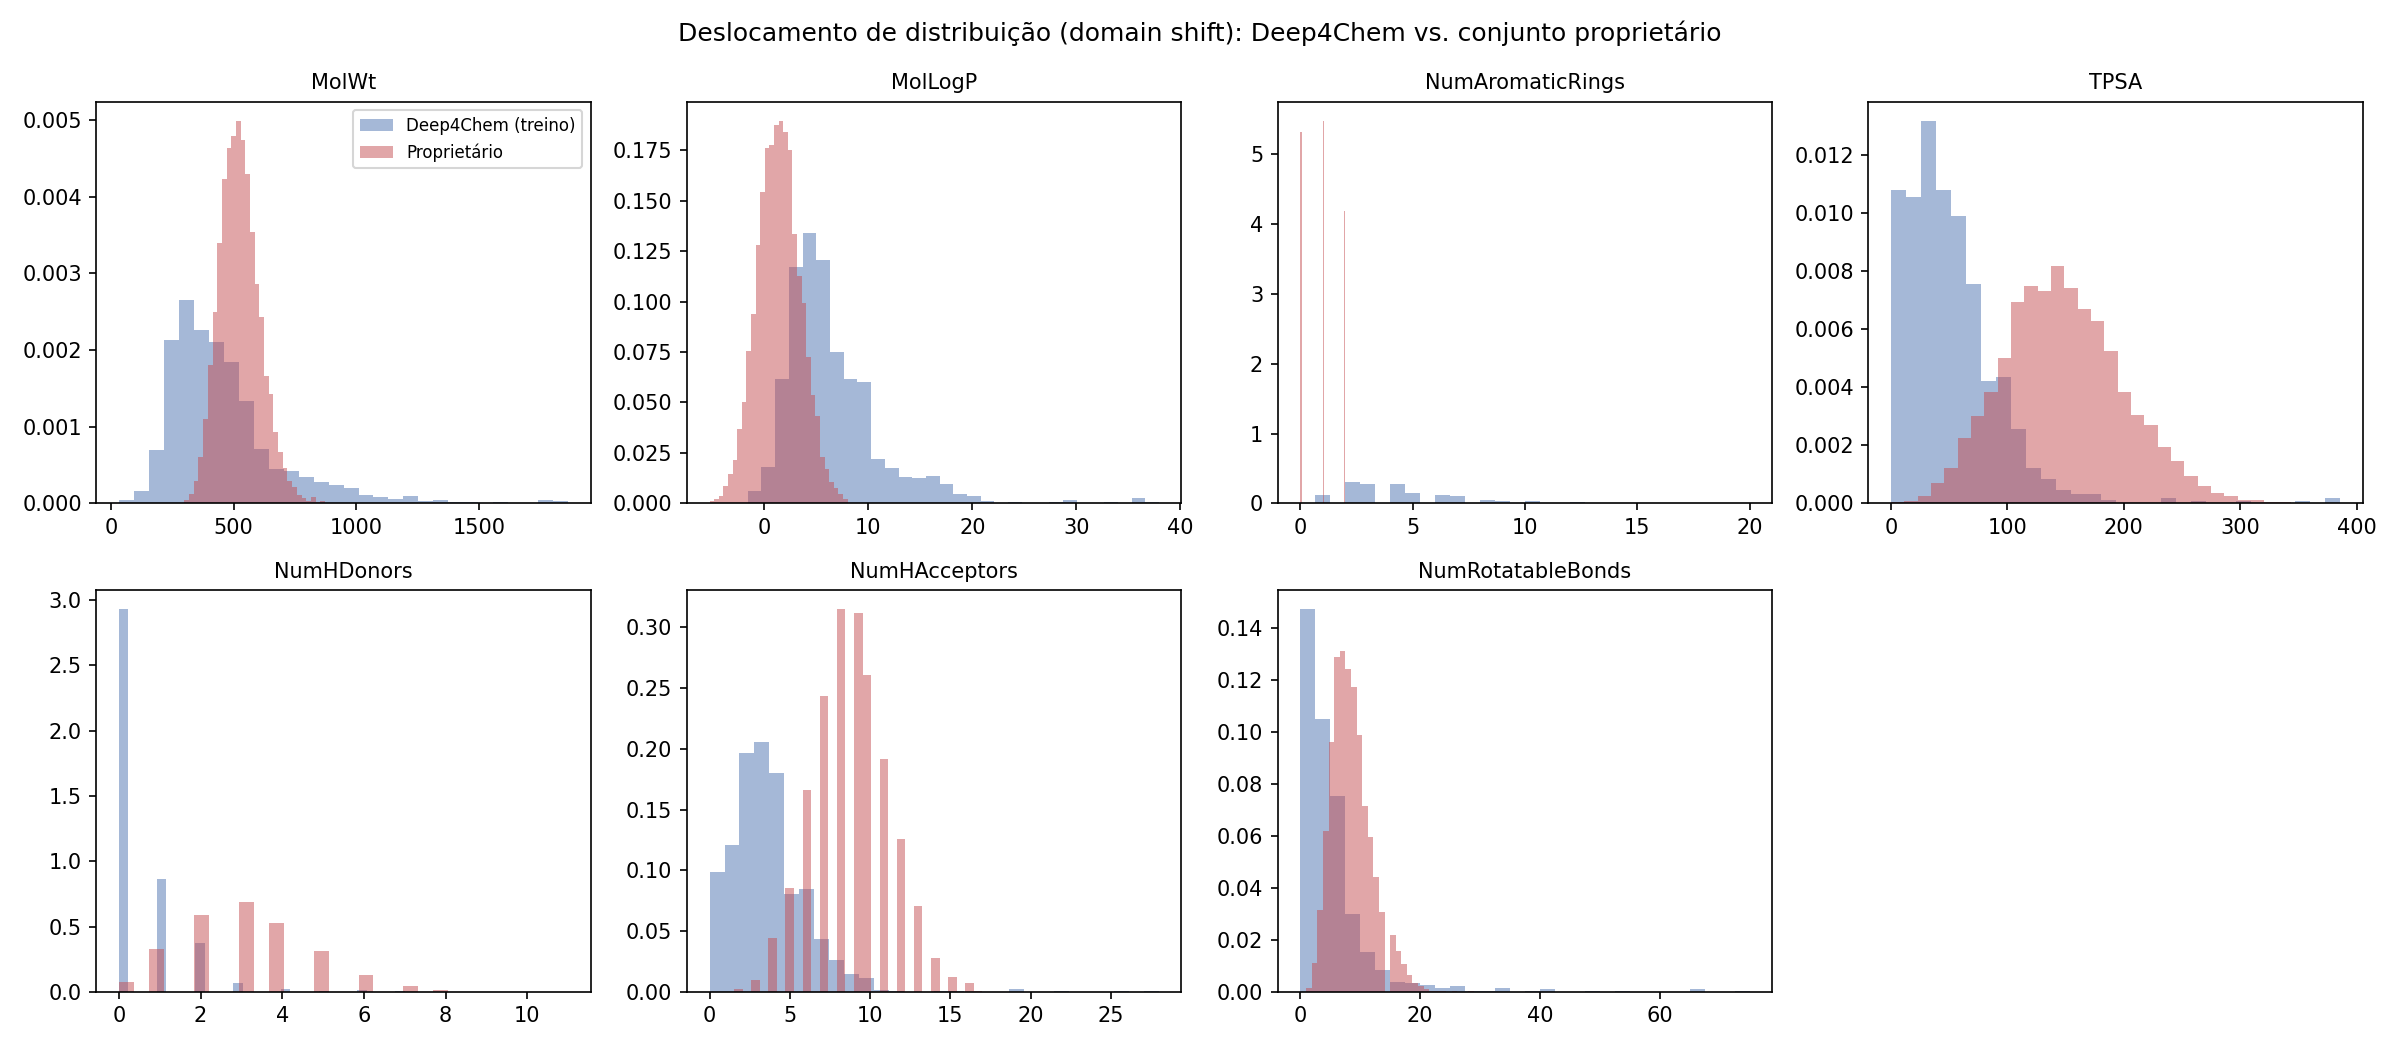
\includegraphics[width=\textwidth]{../resources/figures/domain_shift.png}
\caption{Distribuições sobrepostas de descritores-chave: Deep4Chem (treino) vs. conjunto proprietário -- resultado preliminar.}
\label{fig:domainshift}
\end{figure}

O deslocamento de distribuição é acentuado em todos os sete descritores avaliados (KS entre 0,45 e 0,75, todos com $p < 10^{-180}$). As moléculas proprietárias são, em média, muito mais polares (TPSA quase 3$\times$ maior) e ricas em doadores/aceptores de ligação de hidrogênio, porém possuem \textbf{menos} anéis aromáticos e menor LogP que os cromóforos do Deep4Chem. Como o Deep4Chem é majoritariamente composto por corantes e cromóforos aromáticos conjugados, e o conjunto proprietário parece ocupar uma região mais polar e menos aromática do espaço químico, essa é uma evidência direta de que a transferência do modelo para o conjunto proprietário deve ser tratada com cautela, conforme discutido na Seção 4.

\section{Lições Aprendidas}

\begin{itemize}
  \item \textbf{O que funcionou.} O scaffold split foi implementado e validado corretamente (interseção de scaffolds entre treino e teste igual a zero em todas as execuções). A busca de hiperparâmetros por validação cruzada em grupos de scaffold (\texttt{GroupKFold}) funcionou de forma estável para os três modelos e é reaproveitada, sem alteração de código, entre a execução de validação e a execução completa.
  \item \textbf{Dificuldades de parsing e como foram resolvidas.} Cerca de metade dos SMILES do conjunto proprietário usa aromaticidade explícita com o símbolo \texttt{:} entre átomos não declarados como aromáticos, o que o parser padrão do RDKit rejeita por falha de kekulização. A solução -- reparsear com \texttt{sanitize=False} e pular apenas a etapa \texttt{SANITIZE\_KEKULIZE} -- elevou a taxa de sucesso de $\approx$49\% para 100\% e foi documentada como decisão de design explícita no notebook, não como um contorno silencioso.
  \item \textbf{Um bug sutil de overflow numérico.} Ao calcular o conjunto completo de $\approx$217 descritores RDKit por molécula para o Gradient Boosting, o descritor \texttt{Ipc} (índice de conteúdo de informação) assume valores absurdamente grandes para moléculas maiores, causando \textit{overflow} silencioso ao converter para \texttt{float32} e quebrando o treino do GBM com um \texttt{ValueError} de valores não finitos. A correção foi limitar (\textit{clip}) os descritores a um intervalo numérico seguro antes da conversão de tipo -- um lembrete de que descritores químicos podem ter escalas muito heterogêneas e não devem ser usados sem normalização/tratamento de outliers.
  \item \textbf{Decisões de design que valeriam revisão.} A escolha de um solvente de referência constante (o mais frequente no Deep4Chem, diclorometano) para a Etapa 2, dado que o conjunto proprietário não tem solvente rotulado, é uma simplificação que deveria ser validada com o laboratório ABC Sim -- o solvente efetivamente usado na caracterização das amostras pode ser diferente e influenciar materialmente o $\lambda_{max}$ previsto, dado o efeito solvatocrômico.
  \item \textbf{O deslocamento de distribuição é o maior risco do projeto.} A análise da Seção 3.3 mostrou que o conjunto proprietário ocupa uma região do espaço químico sistematicamente diferente do Deep4Chem (mais polar, menos aromática). Isso significa que, mesmo que o melhor modelo tenha bom desempenho no teste do Deep4Chem, sua confiabilidade ao ser aplicado ao conjunto proprietário não pode ser assumida sem essa análise -- e reforça a importância da quantificação de incerteza (Seção 2.5) para não tratar todas as predições da Etapa 2 com o mesmo grau de confiança.
  \item \textbf{O que será feito diferente / próximos passos.} (i) Executar o notebook completo com \texttt{QUICK\_TEST=False} no Google Colab (GPU) sobre o Deep4Chem inteiro e substituir as Tabelas \ref{tab:comparacao}--\ref{tab:domainshift} pelos resultados finais -- a expectativa é que a Bi-LSTM, que exige mais dados para convergir, melhore de posição relativa ao GBM com o dataset completo; (ii) treinar a extensão opcional D-MPNN (Chemprop) como comparação de estado da arte, caso haja tempo disponível; (iii) comparar quantitativamente o scaffold split com um split aleatório de controle, para reportar o quanto o scaffold split é de fato mais conservador.
\end{itemize}

\section{Conclusão}

Considerando os três critérios definidos para este projeto -- viabilidade do pipeline, desempenho preditivo dos modelos e confiabilidade da aplicação ao conjunto proprietário --, o resultado desta execução preliminar deve ser lido como \textbf{misto, e não como uma resposta definitiva}: parte do trabalho teve resultado \textbf{positivo}, e uma parte central -- a confiabilidade da Etapa 2 -- teve resultado \textbf{negativo}, o que impede, por ora, uma conclusão final sobre a utilidade prática do modelo para o laboratório ABC Sim.

\begin{itemize}
  \item \textbf{Resultado positivo -- viabilidade do pipeline.} O código roda de ponta a ponta sem erros, o \textit{scaffold split} foi implementado e validado corretamente (interseção de scaffolds entre treino e teste sempre igual a zero), a validação cruzada em grupos de scaffold funcionou de forma estável nos três modelos, e o parsing tolerante elevou a cobertura do conjunto proprietário de $\approx$49\% para 100\%. O objetivo de ter um pipeline reprodutível e correto foi integralmente alcançado.
  \item \textbf{Resultado sem resposta significativa (ainda) -- qual arquitetura é a melhor.} Nesta execução reduzida (1.500 registros, poucas épocas), o Gradient Boosting teve o menor MAE (44,5 nm), à frente do MLP (51,1 nm) e, com folga, da Bi-LSTM (81,5 nm) -- o modelo principal proposto no projeto. Isoladamente, esse ranking \textbf{não pode ser interpretado como uma conclusão sobre qual arquitetura é superior}: a Bi-LSTM é treinada do zero, sem pré-treino, e é conhecida por exigir mais dados e épocas para convergir do que os $\approx$1.216 exemplos de treino usados aqui, de modo que seu desempenho fraco é mais provavelmente um artefato do tamanho reduzido da amostra do que uma limitação real da arquitetura. A comparação entre modelos só terá uma resposta significativa após a execução completa (\texttt{QUICK\_TEST=False}) sobre o Deep4Chem inteiro.
  \item \textbf{Resultado negativo -- confiabilidade da aplicação ao conjunto proprietário.} A análise de deslocamento de distribuição apontou diferenças estatisticamente muito significativas ($p < 10^{-180}$) nos sete descritores moleculares comparados, com estatística de Kolmogorov-Smirnov entre 0,45 e 0,75 -- valores altos, que indicam que o conjunto proprietário ocupa uma região do espaço químico substancialmente diferente da usada no treino (mais polar, com mais doadores/aceptores de ligação de hidrogênio e menos aromática). Do ponto de vista do objetivo prático do projeto, este é um resultado \textbf{ruim}: mesmo o Gradient Boosting tendo o melhor MAE no teste do Deep4Chem, essa evidência mostra que sua predição para as 5.974 moléculas do laboratório ABC Sim não deve ser tratada como confiável sem validação experimental adicional. É por isso que a quantificação de incerteza (Seção 2.5) e a filtragem por baixa variância foram incorporadas ao ranking final: o resultado da Etapa 2 deve ser usado como critério de priorização exploratória, não como predição quantitativa validada.
\end{itemize}

Em suma, o projeto demonstrou que a abordagem proposta é \textbf{tecnicamente viável} (pipeline correto, modelos treináveis, incerteza quantificável), mas os números desta execução preliminar \textbf{não permitem afirmar que o modelo generaliza bem para o conjunto proprietário}: o sinal de deslocamento de distribuição é forte o suficiente para justificar cautela, e a comparação entre arquiteturas segue sem resposta significativa até a execução completa. A avaliação honesta do estado atual do projeto é, portanto, que o pipeline \textbf{funciona}, mas a pergunta científica central -- qual modelo é confiável para priorizar síntese no conjunto proprietário -- \textbf{ainda não tem resposta conclusiva}, o que é diferente tanto de um resultado bom quanto de um resultado ruim: é um resultado em aberto, a ser fechado pela execução completa descrita na Seção 4.

\section{Reprodutibilidade}

O código completo do projeto (pré-processamento, treinamento dos modelos, avaliação e aplicação na Etapa 2) está disponível em: \url{https://github.com/crhisangela/ai-ronaldo}.

O repositório inclui o notebook \texttt{main.ipynb}, usado para todos os experimentos, com um flag \texttt{QUICK\_TEST} que alterna entre uma execução reduzida de validação do pipeline (usada para gerar os resultados preliminares desta seção) e a execução completa sobre o Deep4Chem inteiro. O Deep4Chem é baixado automaticamente do Figshare na primeira execução e mantido em cache local (\texttt{resources/deep4chem\_raw/}); o conjunto proprietário é lido de \texttt{resources/banco\_smiles\_aromatizados.parquet}.

\begin{thebibliography}{20}

\bibitem[Adamo and Jacquemin 2013]{adamo2013}
Adamo, C. and Jacquemin, D. (2013).
\newblock The calculations of excited-state properties with time-dependent density functional theory.
\newblock {\em Chemical Society Reviews}, 42(3):845--856.

\bibitem[Bemis and Murcko 1996]{bemis1996}
Bemis, G.~W. and Murcko, M.~A. (1996).
\newblock The properties of known drugs. 1. molecular frameworks.
\newblock {\em Journal of Medicinal Chemistry}, 39(15):2887--2893.

\bibitem[Friedman 2001]{friedman2001}
Friedman, J.~H. (2001).
\newblock Greedy function approximation: A gradient boosting machine.
\newblock {\em The Annals of Statistics}, 29(5):1189--1232.

\bibitem[Gal and Ghahramani 2016]{gal2016}
Gal, Y. and Ghahramani, Z. (2016).
\newblock Dropout as a bayesian approximation: Representing model uncertainty in deep learning.
\newblock In {\em Proceedings of the 33rd International Conference on Machine Learning (ICML)}, pages 1050--1059.

\bibitem[Gilmer et al. 2017]{gilmer2017}
Gilmer, J., Schoenholz, S.~S., Riley, P.~F., Vinyals, O., and Dahl, G.~E. (2017).
\newblock Neural message passing for quantum chemistry.
\newblock In {\em Proceedings of the 34th International Conference on Machine Learning (ICML)}, pages 1263--1272.

\bibitem[Hochreiter and Schmidhuber 1997]{hochreiter1997}
Hochreiter, S. and Schmidhuber, J. (1997).
\newblock Long short-term memory.
\newblock {\em Neural Computation}, 9(8):1735--1780.

\bibitem[Hohenberg and Kohn 1964]{hohenberg1964}
Hohenberg, P. and Kohn, W. (1964).
\newblock Inhomogeneous electron gas.
\newblock {\em Physical Review}, 136(3B):B864--B871.

\bibitem[Joung et al. 2020]{joung2020}
Joung, J.~F., Han, M., Jeong, J., and Park, S. (2020).
\newblock Experimental database of optical properties of organic compounds.
\newblock {\em Scientific Data}, 7:295.

\bibitem[Kohn and Sham 1965]{kohnsham1965}
Kohn, W. and Sham, L.~J. (1965).
\newblock Self-consistent equations including exchange and correlation effects.
\newblock {\em Physical Review}, 140(4A):A1133--A1138.

\bibitem[Lakshminarayanan et al. 2017]{lakshminarayanan2017}
Lakshminarayanan, B., Pritzel, A., and Blundell, C. (2017).
\newblock Simple and scalable predictive uncertainty estimation using deep ensembles.
\newblock In {\em Advances in Neural Information Processing Systems (NeurIPS)}, pages 6402--6413.

\bibitem[Paszke et al. 2019]{paszke2019}
Paszke, A., Gross, S., Massa, F., et~al. (2019).
\newblock Pytorch: An imperative style, high-performance deep learning library.
\newblock In {\em Advances in Neural Information Processing Systems (NeurIPS)}, pages 8026--8037.

\bibitem[Pedregosa et al. 2011]{pedregosa2011}
Pedregosa, F., Varoquaux, G., Gramfort, A., et~al. (2011).
\newblock Scikit-learn: Machine learning in python.
\newblock {\em Journal of Machine Learning Research}, 12:2825--2830.

\bibitem[RDKit 2024]{rdkit2024}
RDKit (2024).
\newblock Rdkit: Open-source cheminformatics.
\newblock \url{https://www.rdkit.org}.

\bibitem[Reichardt 1994]{reichardt1994}
Reichardt, C. (1994).
\newblock Solvatochromic dyes as solvent polarity indicators.
\newblock {\em Chemical Reviews}, 94(8):2319--2358.

\bibitem[Rogers and Hahn 2010]{rogers2010}
Rogers, D. and Hahn, M. (2010).
\newblock Extended-connectivity fingerprints.
\newblock {\em Journal of Chemical Information and Modeling}, 50(5):742--754.

\bibitem[Schuster and Paliwal 1997]{schuster1997}
Schuster, M. and Paliwal, K.~K. (1997).
\newblock Bidirectional recurrent neural networks.
\newblock {\em IEEE Transactions on Signal Processing}, 45(11):2673--2681.

\bibitem[Srivastava et al. 2014]{srivastava2014}
Srivastava, N., Hinton, G., Krizhevsky, A., Sutskever, I., and Salakhutdinov, R. (2014).
\newblock Dropout: A simple way to prevent neural networks from overfitting.
\newblock {\em Journal of Machine Learning Research}, 15(1):1929--1958.

\bibitem[Todeschini and Consonni 2009]{todeschini2009}
Todeschini, R. and Consonni, V. (2009).
\newblock {\em Molecular Descriptors for Chemoinformatics}.
\newblock Wiley-VCH, Weinheim.

\bibitem[Wu et al. 2018]{wu2018}
Wu, Z., Ramsundar, B., Feinberg, E.~N., et~al. (2018).
\newblock Moleculenet: A benchmark for molecular machine learning.
\newblock {\em Chemical Science}, 9(2):513--530.

\bibitem[Yang et al. 2019]{yang2019}
Yang, K., Swanson, K., Jin, W., et~al. (2019).
\newblock Analyzing learned molecular representations for property prediction.
\newblock {\em Journal of Chemical Information and Modeling}, 59:3370--3388.

\end{thebibliography}

\end{document}
